% Appendix G — RQ3 extended results (quarterly trend + native-pool robustness)
% Companion to RQ3 ($\widehat{\rbt^A - \rbt^H}$ in \S\ref{sec:results}). For
% each PR-creation quarter in the analysis window we recompute the within-PR
% DiD under the same stable doubly-engaged cohort definition, separately for
% the (cross-family) Any-AI-vs-human cohort and the (within-family) Claude-
% vs-human cohort. 95\% CIs are analytical (rate-difference scale; two
% independent gaps summed in quadrature). The figure replicates Figure~2 on
% the symmetric (native-only) AI review pool, pooled across all four
% quarters.

\paragraph{Quarterly trend.} The cross-family within-PR DiD ($\widehat{\rbt^A - \rbt^H}$, AI bot reviewer vs.\ human reviewer on AI- vs.\ human-authored PRs) is negative in every quarter of the analysis window --- AI bots are systematically less approving of AI-authored code than humans are --- but its magnitude attenuates from -28.11{}~pp (95\% CI [-41.41{}, -14.81{}]) in 2025-Q2 to -7.11{}~pp ([-9.44{}, -4.77{}]) in 2026-Q1, even as the AI-authored cell grows from 44{} to 1,754{} PRs (Table~\ref{tab:rq3-quarterly}, top); the gap on human-authored PRs is approximately stationary, so the attenuation is driven by AI-authored-PR approval rates rising toward the human reviewer's, not by humans becoming harsher on AI-authored code. The within-family Claude-vs-human DiD is consistent with zero in each quarter for which it is identifiable (the 2025-Q2 cell has zero Claude-authored PRs in the cohort): point estimates are -1.75{}~pp, +20.00{}~pp and +0.86{}~pp for 2025-Q3, 2025-Q4 and 2026-Q1 respectively, with the 2025-Q4 estimate dominated by a Claude-authored cell of 5{} PRs (Table~\ref{tab:rq3-quarterly}, bottom); only 2026-Q1's CI ([-4.27{}, +5.99{}]) is tight enough to rule out anything beyond a small in-family preference, consistent with the pooled within-family result in \S\ref{sec:results}. Restricting the AI review pool to native \texttt{APPROVED}/\texttt{CHANGES\_REQUESTED} review states only --- symmetric with the human side --- shrinks the cross-family AI-authored cell to 2{}, 4{}, 8{} and 71{} PRs across 2025-Q2 $\to$ 2026-Q1 and yields per-quarter DiDs of -39.55{}~pp [-108.88{}, +29.79{}], +2.17{}~pp [-67.17{}, +71.51{}], -11.85{}~pp [-60.14{}, +36.43{}] and +5.29{}~pp [-1.96{}, +12.54{}] respectively --- non-monotone point estimates whose CIs all cross zero, confirming that the headline negative DiD is identified off the regex-parsed verdict pool (\Cref{app:ai-verdict-regex}), not off native review states; the within-family Claude pool under the same restriction collapses to 0{}, 0{}, 0{} and 10{} Claude-authored PRs respectively and is uninformative for all but 2026-Q1 (+0.34{}~pp [-2.38{}, +3.06{}]).

\begin{figure}[h]
    \centering
    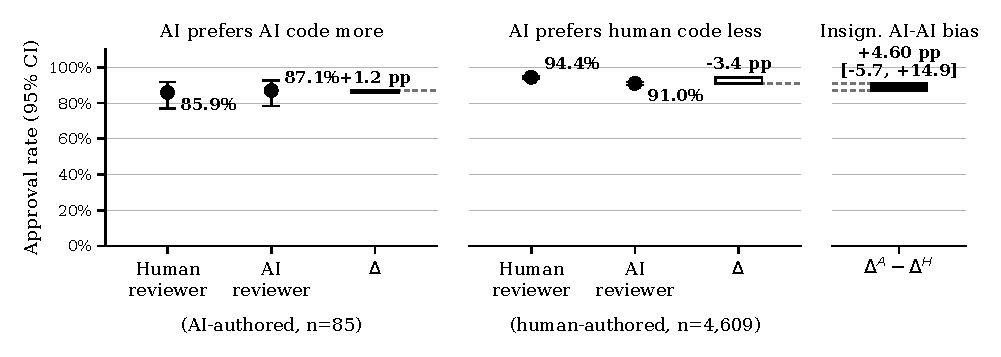
\includegraphics[width=\linewidth]{figures/figure2_withinpr_native.pdf}
    \caption{Within-PR DiD on the dual-review cohort, with the AI review pool restricted to native \texttt{APPROVED} / \texttt{CHANGES\_REQUESTED} review states only (symmetric with the human side). Pooled across the full Apr 2025--Mar 2026 window: 85{} AI-authored and 4,609{} human-authored PRs. Same construction as Figure~\ref{fig:withinpr}. DiD $\widehat{\rbt^A - \rbt^H} = +4.60{}$~pp (95\% CI [-5.73, +14.94]{}) --- the headline negative result in \S\ref{sec:results} does not replicate in this small sample with only explicit review events included: the gap on AI-authored PRs is +1.18{}~pp [95\% CI [-9.11, +11.46]{}] vs.\ a gap of -3.43{}~pp [95\% CI [-4.49, -2.37]{}] on human-authored PRs, and the DiD's CI crosses zero.}
    \label{fig:withinpr-native}
\end{figure}

\begin{figure}[h]
    \centering
    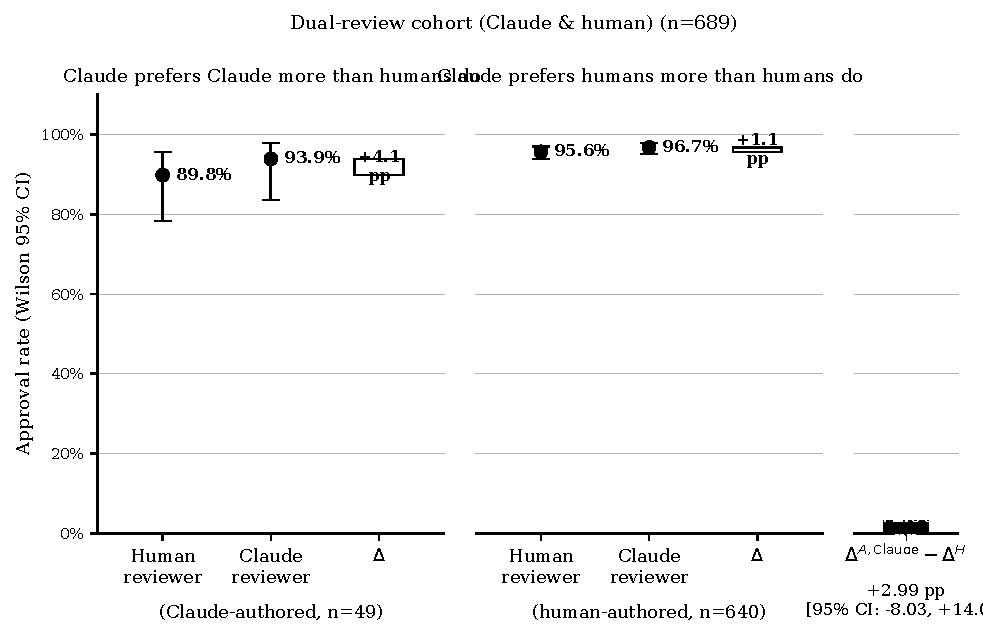
\includegraphics[width=\linewidth]{figures/figure2b_withinfamily_claude.pdf}
    \caption{Within-family check on the dual-review cohort (Claude \& human; 689{} PRs, 49{} Claude-authored). Same construction as Figure~\ref{fig:withinpr}. DiD $\widehat{\rbt^{A,\text{Claude}} - \rbt^H} = +2.99{}$~pp ($p=0.7533${}) --- direction-consistent with a small in-family preference but indistinguishable from zero given the small Claude-authored cell.}
    \label{fig:withinfamily}
\end{figure}

\begin{table}[h]
\centering
\footnotesize
\setlength{\tabcolsep}{4pt}
\begin{tabular}{lrrrr}
\toprule
Quarter & 2025-Q2 & 2025-Q3 & 2025-Q4 & 2026-Q1 \\
\midrule
\multicolumn{5}{l}{\textbf{Cross-family: AI bot reviewer vs.\ human reviewer (RQ3 main)}} \\
PRs in cohort ($n$)               & 6,555{}     & 9,639{}     & 11,708{}     & 18,497{}     \\
\quad AI-authored cell ($n$)      & 44{}   & 141{}   & 462{}   & 1,754{}   \\
\quad H-authored cell ($n$)       & 6,511{}    & 9,498{}    & 11,246{}    & 16,743{}    \\
\multicolumn{5}{l}{\emph{On AI-authored PRs:}} \\
\quad AI rev.\ approval rate         & 9.1\%{}   & 12.8\%{}   & 32.7\%{}   & 20.7\%{}   \\
\quad Human rev.\ approval rate      & 86.4\%{}   & 90.1\%{}   & 90.9\%{}   & 94.0\%{}   \\
\quad gap (pp)                       & -77.27{}   & -77.30{}   & -58.23{}   & -73.32{}   \\
\qquad 95\% CI                       & [-90.50, -64.04]{} & [-84.70, -69.91]{} & [-63.24, -53.21]{} & [-75.52, -71.12]{} \\
\multicolumn{5}{l}{\emph{On human-authored PRs:}} \\
\quad AI rev.\ approval rate         & 44.3\%{}   & 41.1\%{}   & 42.5\%{}   & 26.0\%{}   \\
\quad Human rev.\ approval rate      & 93.5\%{}   & 93.5\%{}   & 92.5\%{}   & 92.2\%{}   \\
\quad gap (pp)                       & -49.16{}   & -52.32{}   & -50.01{}   & -66.21{}   \\
\qquad 95\% CI                       & [-50.51, -47.82]{} & [-53.42, -51.21]{} & [-51.04, -48.97]{} & [-66.99, -65.43]{} \\
DiD ($\widehat{\rbt^A - \rbt^H}$, pp) & -28.11{}  & -24.99{}  & -8.22{}  & -7.11{}  \\
\quad 95\% CI                       & [-41.41, -14.81]{}& [-32.47, -17.51]{}& [-13.34, -3.09]{}& [-9.44, -4.77]{}\\
\midrule
\multicolumn{5}{l}{\textbf{Within-family: Claude reviewer vs.\ human reviewer on Claude- vs.\ human-authored PRs}} \\
PRs in cohort ($n$)               & 47{}    & 59{}    & 81{}    & 502{}    \\
\quad Claude-authored cell ($n$)  & 0{}   & 2{}   & 5{}   & 42{}   \\
\quad H-authored cell ($n$)       & 47{}   & 57{}   & 76{}   & 460{}   \\
\multicolumn{5}{l}{\emph{On Claude-authored PRs:}} \\
\quad Claude rev.\ approval rate     & --{}   & 100.0\%{}   & 40.0\%{}   & 100.0\%{}   \\
\quad Human rev.\ approval rate      & --{}   & 100.0\%{}   & 20.0\%{}   & 97.6\%{}   \\
\quad gap (pp)                       & --{}   & +0.00{}   & +20.00{}   & +2.38{}   \\
\qquad 95\% CI                       & --{} & [+0.00, +0.00]{} & [-35.44, +75.44]{} & [-2.23, +6.99]{} \\
\multicolumn{5}{l}{\emph{On human-authored PRs:}} \\
\quad Claude rev.\ approval rate     & 95.7\%{}   & 93.0\%{}   & 94.7\%{}   & 97.6\%{}   \\
\quad Human rev.\ approval rate      & 97.9\%{}   & 91.2\%{}   & 94.7\%{}   & 96.1\%{}   \\
\quad gap (pp)                       & -2.13{}   & +1.75{}   & +0.00{}   & +1.52{}   \\
\qquad 95\% CI                       & --{} & [-8.14, +11.65]{} & [-7.10, +7.10]{} & [-0.73, +3.78]{} \\
DiD ($\widehat{\rbt^{A,\text{Claude}} - \rbt^H}$, pp) & --{}  & -1.75{}  & +20.00{}  & +0.86{}  \\
\quad 95\% CI                       & --{}& [-11.65, +8.14]{}& [-35.89, +75.89]{}& [-4.27, +5.99]{}\\
\bottomrule
\end{tabular}
\caption{Within-PR DiD (\S\ref{sec:results}) by PR-creation quarter. Top panel: cross-family DiD on the stable doubly-engaged Any-AI-and-human cohort. Bottom panel: within-family DiD on the Claude-and-human cohort, with author restricted to Claude or human (the 2025-Q2 Claude-author cell is empty in the cohort, so its DiD is undefined). The gap on each author-side row is the AI-reviewer approval rate minus the human-reviewer approval rate (in pp); the DiD is the gap on AI-/Claude-authored PRs minus the gap on human-authored PRs. 95\% CIs are analytical (two independent gaps summed in quadrature on the rate-difference scale).}
\label{tab:rq3-quarterly}
\end{table}
